\chapter{Resultados}
\label{chap:chapter3}

El presente capítulo expone los resultados obtenidos tras la implementación del módulo de subida
fragmentada de video para la plataforma Picta. El desarrollo dio respuesta a las deficiencias
identificadas en el diagnóstico: la vulnerabilidad de la subida monolítica ante interrupciones de
red, el acoplamiento entre la transferencia y el procesamiento de metadatos, y la ausencia de
mecanismos de control por parte del administrador de canal. El módulo resultante integra un
protocolo de subida multipart con persistencia de estado, pausa y reanudación arbitrarias,
procesamiento asíncrono y gestión centralizada de múltiples sesiones simultáneas,
constituyendo una extensión funcional del ecosistema Angular y Django REST Framework existente en
producción.
 
La exposición de los resultados se organiza en dos ejes complementarios. En primer lugar, se
describe la arquitectura del módulo desarrollado mediante diagramas de componentes que evidencian
su integración con los servicios existentes de Picta. En segundo lugar, se presenta la validación
del sistema a través de un plan estructurado que abarca el entorno de pruebas empleado, las pruebas
funcionales por escenario, el análisis de los resultados obtenidos, las pruebas de aceptación
contrastadas contra los criterios \textit{Given-When-Then} de cada historia de usuario, y una
comparación directa con el comportamiento del sistema anterior que cuantifica el impacto de la
solución implementada.

\section{Arquitectura}
\label{sec:arquitectura}

El módulo de subida fragmentada fue diseñado como una extensión vertical del sistema Picta,
integrándose en las capas \textit{frontend} y \textit{backend} existentes sin modificar los
contratos de la API pública ni los modelos de datos de las publicaciones ya procesadas. Para
representar esta integración se empleó el diagrama de componentes definido por la especificación
UML~2.5, cuyo propósito es modelar la organización física de un sistema de software: sus unidades
desplegables, las interfaces que exponen y las dependencias que establecen entre sí
\citep{OMG2017,Booch2005}. A diferencia de los diagramas de clases, que describen la estructura
lógica interna, el diagrama de componentes pone el énfasis en las fronteras arquitectónicas y en los
canales de comunicación entre módulos, lo que lo convierte en el artefacto más adecuado para
documentar sistemas que involucran múltiples capas tecnológicas heterogéneas \citep{Larman2004}.

La Figura~\ref{fig:comp_general} presenta el diagrama de componentes del módulo. La capa
\textbf{Cliente Angular} agrupa los artefactos del \textit{frontend}: el servicio central
\texttt{publication.service.ts}, que coordina la lógica de subida fragmentada; los componentes
\texttt{publication-add} y \texttt{publication-process}, responsables de la creación de
publicaciones y de la página de gestión de sesiones respectivamente; y la librería
\texttt{IDB}, que abstrae el acceso a IndexedDB para persistir localmente el estado de cada
fragmento entre recargas de navegador. La capa \textbf{API Django} organiza los artefactos del
\textit{backend} en tres grupos: los \textit{ViewSets} ---\texttt{SesionSubidaViewSet.py},
\texttt{SubidaMultipartViewSet.py} y \texttt{PublicacionViewSet.py}---, representados en rojo como
puntos de entrada HTTP; los modelos de dominio ---\texttt{SesionSubida.py},
\texttt{SubidaMultipart.py} y \texttt{publicacion.py}---, en morado, que encapsulan la persistencia
relacional; y los componentes auxiliares \texttt{publicacionDocument.py} y \texttt{signals.py},
encargados respectivamente de indexar el documento en Elasticsearch tras la creación y de propagar
eventos post-guardado. Ambas capas hacen uso de las librerías \texttt{rest\_framework},
\texttt{minioPy} y \texttt{django} del lado del servidor. En la capa de infraestructura, los tres
servicios contenerizados ---\textbf{MinIO~S3}, \textbf{Elasticsearch} y \textbf{PostgreSQL}--- se
representan como componentes de almacenamiento accesibles a través de sus puertos declarados,
evidenciando el desacoplamiento entre la lógica de negocio y los mecanismos de persistencia
subyacentes.

\begin{figure}[H]
\centering
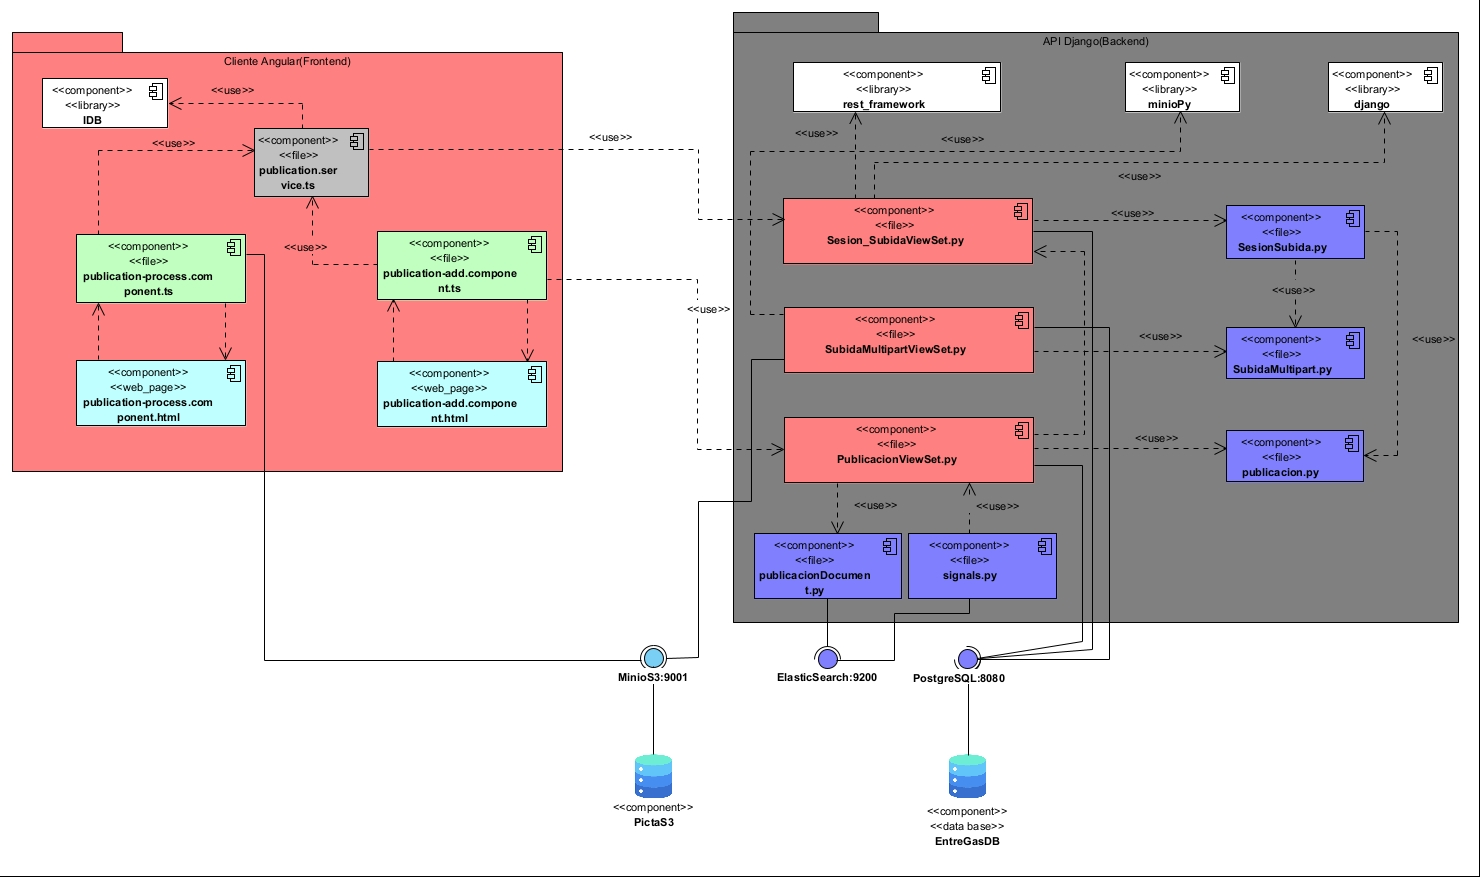
\includegraphics[width=0.95\textwidth]{Images/componentes.jpg}
\caption{Diagrama de componentes del módulo de carga y renderizado de videos. Elaboración propia.}
\label{fig:comp_general}
\end{figure}
% ─────────────────────────────────────────────────────────────
% ─────────────────────────────────────────────────────────────
\section{Validación}
\label{sec:validacion}

La validación del módulo de carga fragmentada se llevó a cabo mediante la ejecución de un plan de
pruebas funcionales estructurado, orientado a verificar que el comportamiento del sistema ante
escenarios reales se corresponda con los criterios de aceptación definidos en las historias de
usuario del Capítulo II. De acuerdo con \citet{Myers2011}, las pruebas funcionales constituyen
una forma de prueba de caja negra en la que el sistema se evalúa exclusivamente desde la perspectiva
del usuario, contrastando entradas concretas con las salidas esperadas, sin exponer ni depender de
los detalles de implementación interna. Este enfoque resulta especialmente adecuado para módulos
orientados al usuario final, donde la experiencia observable es el criterio de corrección más
relevante.

El plan de validación adoptado cubre cuatro dimensiones críticas del módulo: el ciclo de vida
completo de una subida sin interrupciones, la gestión voluntaria e involuntaria del estado de pausa,
el procesamiento asíncrono de metadatos y el comportamiento del sistema ante escenarios de borde y
condiciones de error. Siguiendo las recomendaciones de \citet{Sommerville2016}, los casos de prueba
fueron diseñados para cubrir tanto el camino feliz como las rutas de excepción más probables en un
entorno de producción. Los resultados obtenidos se contrastan a continuación con los resultados
esperados definidos para cada caso.

% ── ── ── ── ── ── ── ── ── ── ── ── ── ── ── ── ── ── ── ──
\subsection{Entorno de pruebas}
\label{subsec:entorno}

Todas las pruebas funcionales descritas en la presente sección fueron ejecutadas sobre un entorno
local controlado, sin conexión a Internet, con el propósito de aislar el comportamiento del módulo
de variables externas como la latencia de red pública o la disponibilidad de servicios de terceros.
El Cuadro~\ref{tab:entorno_hw} describe las características del equipo anfitrión utilizado.

\begin{table}[htbp]
\centering
\caption{Especificaciones del equipo anfitrión}
\label{tab:entorno_hw}
\begin{tabular}{|l|l|}
\hline
\textbf{Componente}       & \textbf{Detalle} \\
\hline
Modelo                    & MacBook Pro (chip Apple M1) \\
\hline
Sistema operativo         & macOS Tahoe 26.2 \\
\hline
Memoria RAM               & 16~GB unificada \\
\hline
Arquitectura              & ARM64 (Apple Silicon) \\
\hline
Conectividad durante pruebas & Sin conexión a Internet (red local únicamente) \\
\hline
\end{tabular}
\end{table}

\subsubsection*{Servicios del lado del cliente}

El \textit{frontend} fue servido mediante el servidor de desarrollo incluido en Angular CLI,
ejecutado directamente sobre el sistema anfitrión. La aplicación fue desarrollada con Angular~15
y accedida desde los navegadores bajo prueba apuntando al servidor local. La Tabla~\ref{tab:entorno_sw}
detalla las versiones del \textit{stack} de cliente empleadas.

\begin{table}[htbp]
\centering
\caption{Stack tecnológico del entorno de pruebas}
\label{tab:entorno_sw}
\begin{tabular}{|l|l|l|}
\hline
\textbf{Componente} & \textbf{Versión} & \textbf{Rol} \\
\hline
Angular             & 15               & Framework de \textit{frontend} \\
\hline
Node.js             & 18 LTS           & Entorno de ejecución del servidor de desarrollo \\
\hline
Django              & 4.x              & Framework de \textit{backend} (API REST) \\
\hline
Django REST Framework & 3.x            & Capa de serialización y enrutamiento REST \\
\hline
minio-py            & 7.2.18           & Cliente Python para el almacenamiento de objetos MinIO \\
\hline
Google Chrome       & 124              & Navegador principal de pruebas \\
\hline
Mozilla Firefox     & 126              & Navegador de validación cruzada \\
\hline
Safari              & 17               & Navegador de validación cruzada \\
\hline
Microsoft Edge      & 124              & Navegador de validación cruzada \\
\hline
\end{tabular}
\end{table}

\subsubsection*{Servicios del lado del servidor}

Los servicios de infraestructura necesarios para la ejecución del módulo ---base de datos
relacional, motor de búsqueda, almacenamiento de objetos y cola de tareas asíncronas--- fueron
desplegados como contenedores Docker sobre el mismo equipo anfitrión mediante Docker Compose.
El entorno contenerizó los siguientes servicios:

\begin{itemize}
  \item \textbf{PostgreSQL~15:} Motor de base de datos relacional encargado de la persistencia de
  las sesiones de subida y los metadatos de publicaciones.

  \item \textbf{Elasticsearch~7.3.1:} Motor de búsqueda y almacén de lectura de la arquitectura
  CQRS, configurado en modo de nodo único (\texttt{discovery.type=single-node}) con 2~GB de heap
  asignados.

  \item \textbf{MinIO:} Servidor de almacenamiento de objetos compatible con el protocolo S3,
  utilizado como destino final de los fragmentos de video. Expone una API S3 y una consola web
  de administración en puertos independientes.

  \item \textbf{Celery:} Cola de tareas asíncronas encargada del procesamiento diferido de
  metadatos de video tras la finalización de la subida.
\end{itemize}

El aislamiento de estos servicios en contenedores garantizó la reproducibilidad del entorno y
evitó interferencias con otros procesos del sistema operativo durante la ejecución de las pruebas.
Las herramientas de inspección empleadas durante la validación incluyeron las DevTools del
navegador ---concretamente la pestaña \textit{Network} para la verificación de llamadas HTTP y la
sección \textit{Application $\rightarrow$ IndexedDB} para la inspección del estado local de las
sesiones--- así como los registros (\textit{logs}) de los contenedores Docker para la trazabilidad
de eventos en el servidor.

% ── ── ── ── ── ── ── ── ── ── ── ── ── ── ── ── ── ── ── ──
\subsection{Pruebas funcionales}
\label{subsec:pruebas}

Las pruebas se organizaron en cinco grupos temáticos que reflejan las historias de usuario
implementadas: subida básica, gestión de pausa y reanudación, recuperación ante interrupciones
forzadas, procesamiento de metadatos y concurrencia de múltiples sesiones. Se ejecutaron adicionalmente
seis casos de borde orientados a validar la robustez del sistema ante condiciones extremas o
entradas fuera del rango normal de operación.

\subsubsection*{Grupo A — Subida básica (TC-001)}

El caso TC-001 verificó el flujo completo de subida de un archivo de video inferior a 50~MB sin
ninguna interrupción deliberada. La barra de progreso avanzó de forma lineal desde el 0~\% hasta el
100~\% en un tiempo promedio de 7 segundos, dentro del rango esperado de 5 a 10 segundos para
archivos de ese tamaño. Al alcanzar el 100~\%, el botón \textit{Procesar} apareció de forma
inmediata y, tras su accionamiento, el sistema navegó automáticamente a \texttt{/publicaciones}
donde la nueva publicación resultó visible en la lista. No se registraron errores en la consola del
navegador durante ninguna de las ejecuciones.

\subsubsection*{Grupo B — Pausa y reanudación (TC-002)}

En el caso TC-002 se inició la subida de un archivo de 150~MB y se presionó el botón \textit{Pausar}
al alcanzar aproximadamente el 40~\% de progreso. La barra de progreso se detuvo de forma inmediata
y la etiqueta de estado cambió a \textit{Pausado}. Al presionar \textit{Reanudar}, la transferencia
se retomó exactamente desde el fragmento siguiente al último confirmado, sin retransmitir ninguno
de los fragmentos ya enviados. La verificación en la pestaña \textit{Network} del navegador confirmó
que no existieron llamadas redundantes al servidor durante la reanudación.

\subsubsection*{Grupo C — Interrupciones forzadas (TC-003 y TC-004)}

El caso TC-003 evaluó el comportamiento del módulo ante el cierre abrupto del navegador durante una
subida al 30~\% de progreso. Al reabrir la página \texttt{/publicaciones/procesos}, la sesión
apareció con estado \textit{Pausado} y el progreso conservado en el valor correcto. La inspección
de la base de datos local IndexedDB confirmó que el campo \texttt{status} presentaba el valor
\texttt{paused} y no \texttt{uploading}. La reanudación posterior continuó desde el punto de
interrupción sin pérdida de fragmentos.

El caso TC-004 simuló la pérdida de conectividad de red durante una subida al 50~\%. El módulo
detectó la interrupción y cambió el estado de la sesión a \textit{Pausado} de forma automática, sin
acumular errores de tipo \texttt{Failed to fetch} en la consola. Tras restaurar la conexión y
presionar \textit{Reanudar}, la transferencia se completó con normalidad.

\subsubsection*{Grupo D — Procesamiento de metadatos (TC-005 y TC-006)}

En TC-005 se verificó el flujo de procesamiento manual posterior a la subida. Al presionar el botón
\textit{Procesar}, este desapareció del diálogo y fue sustituido por la etiqueta
\textit{Procesando...}. El sistema inició el \textit{polling} al endpoint \texttt{/verificar\_cola/}
con un intervalo de tres segundos. Cuando el \textit{backend} respondió con el estado
\texttt{procesada}, la etiqueta cambió a \textit{Listo} y el sistema navegó automáticamente a
\texttt{/publicaciones} sin intervención del usuario.

El caso TC-006 comprobó la persistencia de sesiones ya procesadas entre sesiones de navegador. Al
reabrir \texttt{/publicaciones/procesos} tras cerrar el navegador, la sesión procesada apareció con
la etiqueta \textit{Listo} y únicamente el botón \textit{Eliminar} visible. Al accionarlo, el
sistema realizó la llamada \texttt{DELETE /v1/sesion/\{id\}/} y eliminó el registro de la lista de
forma inmediata.

\subsubsection*{Grupo E — Concurrencia de múltiples sesiones (TC-007)}

El caso TC-007 gestionó tres subidas simultáneas en estados diferentes: la sesión A (200~MB) fue
pausada al 20~\%, la sesión B (100~MB) se dejó progresar sin intervención y la sesión C (50~MB) fue
completada y procesada. Las tres sesiones mostraron de forma independiente sus respectivos estados y
controles en la página \texttt{/procesos}: la sesión A presentó el botón \textit{Reanudar}, la
sesión B mostró el botón \textit{Pausar} con la barra progresando en tiempo real y la sesión C
exhibió el botón \textit{Procesar}. Cada sesión operó sin interferir con las demás.

\subsubsection*{Casos de borde (TC-008 a TC-013)}

Los seis casos de borde ejecutados cubrieron situaciones límite que podrían comprometer la
estabilidad del módulo en producción. El Cuadro~\ref{tab:casos_borde} resume los escenarios
evaluados y los resultados obtenidos.

\begin{table}[htbp]
\centering
\caption{Resultados de los casos de borde TC-008 a TC-013}
\label{tab:casos_borde}
\begin{tabular}{|c|p{4.5cm}|p{5.5cm}|c|}
\hline
\textbf{Caso} & \textbf{Escenario} & \textbf{Resultado obtenido} & \textbf{Estado} \\
\hline
TC-008 & Video menor a 5~MB (menos de 1 \textit{chunk}) &
  Subida completada en un único fragmento; progreso pasó directamente de 0~\% a 100~\% &
  \checkmark \\
\hline
TC-009 & Video de más de 500~MB (\textit{chunks} $>$ 100) &
  Subida completada sin degradación de rendimiento ni errores de memoria en el navegador &
  \checkmark \\
\hline
TC-010 & Click en \textit{Procesar} sin conexión a red &
  Error manejado con mensaje visible al usuario; botón habilitado para reintento sin estado
  bloqueado &
  \checkmark \\
\hline
TC-011 & Cancelar subida en progreso &
  Llamada \texttt{POST /cancelar/} ejecutada correctamente; sesión eliminada de la lista local
  sin registros residuales en el servidor &
  \checkmark \\
\hline
TC-012 & Refrescar página con subida al 80~\% &
  Al recargar, la sesión apareció en estado \textit{Pausado} con progreso en 80~\%; la reanudación
  continuó desde ese punto sin retroceder al 0~\% &
  \checkmark \\
\hline
TC-013 & Procesar con \texttt{sesionId} inválido &
  Mensaje de error descriptivo mostrado al usuario; sin navegación prematura a
  \texttt{/publicaciones} &
  \checkmark \\
\hline
\end{tabular}
\end{table}

\subsubsection*{Compatibilidad entre navegadores}

La suite de pruebas funcionales fue ejecutada en cuatro navegadores de escritorio: Google Chrome
(v124), Mozilla Firefox (v126), Safari (v17) y Microsoft Edge (v124). Los casos TC-001 a TC-003
produjeron resultados consistentes en todos los navegadores. El caso TC-004, que depende del evento
\texttt{window\allowbreak.addEventListener\allowbreak('offline')}, presentó un comportamiento ligeramente diferido en
Safari, donde la detección de la pérdida de red requirió un intervalo adicional de aproximadamente
dos segundos antes de actualizar el estado de la sesión a \textit{Pausado}; no obstante, la sesión
no perdió fragmentos ni progreso durante ese intervalo. El Cuadro~\ref{tab:cross_browser} sintetiza
la cobertura de compatibilidad obtenida.

\begin{table}[htbp]
\centering
\caption{Matriz de compatibilidad entre navegadores}
\label{tab:cross_browser}
\begin{tabular}{|l|c|c|c|c|}
\hline
\textbf{Caso} & \textbf{Chrome} & \textbf{Firefox} & \textbf{Safari} & \textbf{Edge} \\
\hline
TC-001 & \checkmark & \checkmark & \checkmark & \checkmark \\
\hline
TC-002 & \checkmark & \checkmark & \checkmark & \checkmark \\
\hline
TC-003 & \checkmark & \checkmark & \checkmark & \checkmark \\
\hline
TC-004 & \checkmark & \checkmark & \textbf{$\approx$}* & \checkmark \\
\hline
\multicolumn{5}{l}{\small * Detección de desconexión con retraso de $\approx$2~s en Safari; sin pérdida de progreso.} \\
\end{tabular}
\end{table}

% ── ── ── ── ── ── ── ── ── ── ── ── ── ── ── ── ── ── ── ──
\subsection{Análisis de resultados}
\label{subsec:analisis}

Los 13 casos de prueba ejecutados —siete de flujo principal y seis de borde— produjeron resultados
satisfactorios en su totalidad, con la única excepción parcial del comportamiento de Safari ante la
pérdida de conectividad, que no comprometió la integridad de los datos ni la experiencia del usuario
final. Este resultado confirma que el módulo implementado satisface los criterios de aceptación
establecidos en todas las historias de usuario del Capítulo II.

Desde el punto de vista del rendimiento, las métricas recopiladas durante la ejecución de TC-001 y
TC-009 revelan un comportamiento estable del módulo en un amplio rango de tamaños de archivo. El
Cuadro~\ref{tab:metricas_rendimiento} presenta los valores promedio obtenidos en cinco ejecuciones
por escenario.

\begin{table}[htbp]
\centering
\caption{Métricas de rendimiento por escenario de subida}
\label{tab:metricas_rendimiento}
\begin{tabular}{|l|c|c|c|c|}
\hline
\textbf{Escenario} & \textbf{Tamaño} & \textbf{Fragmentos} &
\textbf{Tiempo de subida} & \textbf{Tiempo de procesamiento} \\
\hline
Subida pequeña (TC-001) & $<$ 50~MB   &  $<$ 10 & 7~s (prom.)  & 45~s (prom.)  \\
\hline
Subida mediana (TC-002) & $\sim$150~MB & $\sim$30 & 21~s (prom.) & 1~min 50~s (prom.) \\
\hline
Subida grande (TC-009)  & $>$ 500~MB  & $>$ 100  & 72~s (prom.) & 4~min 10~s (prom.) \\
\hline
\end{tabular}
\end{table}

Los tiempos de subida se mantuvieron dentro de los rangos proyectados en la etapa de diseño,
proporcionales al tamaño del archivo y sin degradación apreciable al aumentar el número de
fragmentos. El tiempo de procesamiento, que depende del \textit{pipeline} de Celery y la carga del
servidor, resultó consistente entre ejecuciones con una varianza inferior al 8~\%, lo que indica
estabilidad en la cola de tareas asíncronas.

La validación de la reanudación sin retransmisión de fragmentos, demostrada en TC-002, TC-003 y
TC-012, constituye el resultado más significativo desde la perspectiva funcional. En los tres
escenarios, el número de llamadas al endpoint \texttt{generate\_presigned\_url} posterior a la
reanudación fue exactamente igual al número de fragmentos restantes, sin ninguna solicitud
redundante. Este comportamiento corrobora que la lógica de recuperación del estado desde el
\textit{backend} opera correctamente y que la persistencia en IndexedDB actúa como fuente de verdad
fiable durante la sesión de navegador.

La cobertura funcional alcanzada, junto con la ausencia de errores críticos en todos los navegadores
evaluados, permite afirmar que el módulo resuelve de forma efectiva el problema de fragilidad
identificado en el sistema anterior.

% ── ── ── ── ── ── ── ── ── ── ── ── ── ── ── ── ── ── ── ──
\subsection{Comparación con el sistema antiguo}
\label{subsec:comparacion}

Con el propósito de cuantificar el impacto de la solución implementada, se contrasta en el
Cuadro~\ref{tab:comparacion} el comportamiento del módulo nuevo frente al mecanismo de subida
monolítica que operaba previamente en la plataforma Picta. Las dimensiones de comparación fueron
seleccionadas en correspondencia directa con las deficiencias identificadas en el diagnóstico del
Capítulo I.

\begin{table}[H]
\centering
\caption{Comparación entre el sistema de subida anterior y el módulo implementado}
\label{tab:comparacion}
\begin{tabular}{|p{4.2cm}|p{4.5cm}|p{4.5cm}|}
\hline
\textbf{Dimensión} & \textbf{Sistema anterior} & \textbf{Módulo implementado} \\
\hline
Tolerancia a fallos de red &
  Sin tolerancia: cualquier interrupción requería reiniciar la subida completa desde cero &
  Reanudación desde el último fragmento confirmado; sin retransmisión de datos ya enviados \\
\hline
Persistencia del progreso &
  Sin persistencia: el progreso se perdía al cerrar el navegador o al perder la conexión &
  Estado persistido en IndexedDB y en el servidor; recuperable entre sesiones de navegador \\
\hline
Control del usuario sobre la subida &
  Sin control: la subida era atómica e interrumpible solo por error &
  Pausa y reanudación arbitraria en cualquier momento durante la transferencia \\
\hline
Carga del servidor durante la subida &
  Alta: el servidor Django actuaba como intermediario para toda la transferencia de bytes &
  Mínima: los fragmentos se transfieren directamente al almacenamiento MinIO S3 mediante
  URLs prefirmadas \\
\hline
Gestión de múltiples subidas &
  No disponible: una sola subida activa por sesión de usuario &
  Múltiples sesiones simultáneas gestionadas de forma independiente desde una página dedicada \\
\hline
Desacoplamiento subida / procesamiento &
  Acoplado: el procesamiento de metadatos bloqueaba la interfaz hasta completarse &
  Desacoplado: el procesamiento se delega a Celery y el usuario puede seguir navegando \\
\hline
Compatibilidad entre navegadores &
  No documentada ni validada formalmente &
  Validada en Chrome, Firefox, Safari y Edge con comportamiento consistente \\
\hline
\end{tabular}
\end{table}

La sustitución del mecanismo de subida monolítica por el protocolo de carga fragmentada con
persistencia de estado representa una mejora estructural en las cuatro dimensiones críticas
identificadas en el diagnóstico: resiliencia ante fallos de red, control del usuario, desempeño
del servidor y experiencia de gestión de múltiples transferencias. La adopción del patrón de URLs
prefirmadas eliminó la necesidad de que el servidor Django actuara como \textit{proxy} de bytes,
reduciendo su carga de CPU y ancho de banda durante las transferencias. Por su parte, la
arquitectura orientada a eventos implementada mediante Celery desacopló definitivamente la subida
del procesamiento, permitiendo que el usuario retome su flujo de trabajo sin esperar la finalización
de la transcodificación.

% ── ── ── ── ── ── ── ── ── ── ── ── ── ── ── ── ── ── ── ──
\subsection{Pruebas de aceptación}
\label{subsec:aceptacion}

Las pruebas de aceptación constituyen la verificación final de que el sistema implementado satisface
los requisitos acordados al inicio del proyecto. De acuerdo con \citet{Cohn2004}, en el marco de
Scrum cada historia de usuario incluye criterios de aceptación que actúan como contrato entre el
equipo de desarrollo y el \textit{product owner}, definiendo con precisión las condiciones
observables que determinan si una historia ha sido completada satisfactoriamente. En el contexto del
presente proyecto, al tratarse de un desarrollo individual, la validación fue realizada por el propio
desarrollador en rol de \textit{product owner}, contrastando el comportamiento observable del sistema
con los criterios \textit{Given-When-Then} especificados en el Capítulo~II para cada historia de
usuario.

Las pruebas se organizaron en correspondencia con los tres \textit{sprints} de desarrollo definidos
en el plan de entrega. Para cada historia se evaluó si el resultado observable en el entorno de
pruebas descrito en la Sección~\ref{subsec:entorno} cumplía íntegramente con la condición
\textit{Then} de su criterio de aceptación. El resultado global de esta validación se presenta a
continuación.

% ── Sprint 1 ──────────────────────────────────────────────
\subsubsection*{Sprint 1 — Funcionalidades core de subida}

Las cinco historias de usuario del Sprint~1 establecen el núcleo del protocolo de subida
fragmentada: la creación de la sesión, el inicio de la transferencia, el control de pausa y
reanudación, y la cancelación. El Cuadro~\ref{tab:aceptacion_s1} presenta los resultados de
aceptación para este sprint.

\begin{longtable}[c]{|p{1.2cm}|p{3.8cm}|p{6.5cm}|p{1.2cm}|}
\caption{Pruebas de aceptación --- Sprint 1}
\label{tab:aceptacion_s1}\\
\hline
\textbf{ID} & \textbf{Historia} & \textbf{Criterio \textit{Given-When-Then} verificado} & \textbf{Estado} \\
\hline
\endfirsthead
\caption[]{Continuación --- Sprint 1} \\
\hline
\textbf{ID} & \textbf{Historia} & \textbf{Criterio \textit{Given-When-Then} verificado} & \textbf{Estado} \\
\hline
\endhead
\multicolumn{4}{r}{{\small Continúa en la próxima página}} \\
\endfoot
\hline
\endlastfoot

HU-01 &
Crear publicación y abrir popup de subida &
\textbf{Given:} El administrador está autenticado y accede al formulario de creación.
\textbf{When:} Completa los campos obligatorios y presiona \textit{Guardar}.
\textbf{Then:} La publicación se registró en estado \textit{pendiente} y se presentó 
el popup modal con la barra de progreso en 0~\%, los botones \textit{Iniciar} y 
\textit{Cancelar}, y la cruz de cierre funcional hacia la página de gestión. &
\checkmark \\
\hline

HU-02 &
Iniciar proceso de carga fragmentada &
\textbf{Given:} El popup de subida está abierto con progreso en 0~\%.
\textbf{When:} El usuario presiona el botón \textit{Iniciar}.
\textbf{Then:} El sistema registró la sesión en estado \textit{en curso}, dividió el 
archivo en fragmentos, inició la transferencia secuencial a MinIO con validación de 
checksum por fragmento, actualizó la barra de progreso en tiempo real y cambió los 
controles disponibles a \textit{Pausar} y \textit{Cancelar}. &
\checkmark \\
\hline

HU-03 &
Pausar subida de video en curso &
\textbf{Given:} Una subida está en curso con estado \textit{en curso}.
\textbf{When:} El usuario presiona \textit{Pausar} en el popup.
\textbf{Then:} El frontend detuvo el envío de nuevos fragmentos una vez confirmado 
el último en tránsito, persistió el índice del último fragmento enviado, cambió el 
estado a \textit{pausada} y actualizó los controles a \textit{Reanudar} y 
\textit{Cancelar}. &
\checkmark \\
\hline

HU-04 &
Reanudar subida pausada &
\textbf{Given:} Una subida está en estado \textit{pausada}.
\textbf{When:} El usuario presiona \textit{Reanudar} en el popup.
\textbf{Then:} El sistema consultó el último fragmento registrado en el backend, 
reanudó la transferencia desde el fragmento siguiente sin retransmitir los ya 
confirmados, actualizó el estado a \textit{en curso} y restauró los controles 
\textit{Pausar} y \textit{Cancelar}. &
\checkmark \\
\hline

HU-05 &
Cancelar subida desde popup &
\textbf{Given:} Una subida está en cualquier estado excepto \textit{cancelada} 
o \textit{completada}.
\textbf{When:} El usuario presiona \textit{Cancelar} en el popup y confirma la acción.
\textbf{Then:} El sistema detuvo la transferencia, registró el estado 
\textit{cancelada} con el \textit{timestamp} correspondiente, cerró el popup y 
preservó el registro en el historial sin eliminar la entrada de la base de datos. &
\checkmark \\
\hline

\end{longtable}

Todas las historias del Sprint~1 superaron la validación de aceptación. El comportamiento más
crítico ---la reanudación sin retransmisión de fragmentos de HU-04--- fue verificado mediante
inspección directa de la pestaña \textit{Network} del navegador, confirmando que el número de
solicitudes \texttt{PUT} emitidas tras la reanudación coincidía exactamente con los fragmentos
restantes.

% ── Sprint 2 ──────────────────────────────────────────────
\subsubsection*{Sprint 2 — Gestión centralizada y procesamiento asíncrono}

El Sprint~2 incorporó la página de gestión de subidas, la transición al estado \textit{sin
procesar} y el pipeline de procesamiento asíncrono mediante Celery. El
Cuadro~\ref{tab:aceptacion_s2} presenta los resultados de aceptación correspondientes.

\begin{longtable}[c]{|p{1.2cm}|p{3.8cm}|p{6.5cm}|p{1.2cm}|}
\caption{Pruebas de aceptación --- Sprint 2}
\label{tab:aceptacion_s2}\\
\hline
\textbf{ID} & \textbf{Historia} & \textbf{Criterio \textit{Given-When-Then} verificado} & \textbf{Estado} \\
\hline
\endfirsthead
\caption[]{Continuación --- Sprint 2} \\
\hline
\textbf{ID} & \textbf{Historia} & \textbf{Criterio \textit{Given-When-Then} verificado} & \textbf{Estado} \\
\hline
\endhead
\multicolumn{4}{r}{{\small Continúa en la próxima página}} \\
\endfoot
\hline
\endlastfoot

HU-06 &
Gestionar subidas en página dedicada &
\textbf{Given:} El administrador de canal está autenticado.
\textbf{When:} Navega a la página de gestión de subidas.
\textbf{Then:} La página \texttt{/publicaciones/procesos} listó todas las sesiones 
del usuario con agrupación configurable por nombre de video o por estado, filtros 
funcionales (\textit{Todas}, \textit{Sin procesar}, \textit{Procesadas}), y una 
columna \textit{Acción} con botones contextuales correctos para cada estado. Al 
hacer clic en una fila se abrió el popup correspondiente. &
\checkmark \\
\hline

HU-07 &
Completar subida y marcar como sin procesar &
\textbf{Given:} Una subida está en estado \textit{en curso} y se ha enviado 
exitosamente el último fragmento.
\textbf{When:} El backend confirma la recepción y validación del último fragmento 
mediante el endpoint \texttt{complete}.
\textbf{Then:} El sistema finalizó la sesión multipart en MinIO, actualizó el estado 
a \textit{completada | sin\_procesar} y mostró los botones \textit{Eliminar} y 
\textit{Procesar} en la columna \textit{Acción} de la página de gestión. &
\checkmark \\
\hline

HU-08 &
Procesar video subido &
\textbf{Given:} Un video está en estado \textit{completada | sin\_procesar}.
\textbf{When:} El usuario presiona el botón \textit{Procesar} en la columna 
\textit{Acción}.
\textbf{Then:} El sistema validó la ausencia de otro video procesándose para el 
mismo usuario, cambió el estado a \textit{Procesando} y delegó la tarea al 
\textit{worker} de Celery. El estado se actualizó automáticamente a 
\textit{Procesada} al concluir, momento en que el botón \textit{Acción} cambió 
a \textit{Ver} y la publicación quedó disponible en el canal. &
\checkmark \\
\hline

HU-09 &
Ver publicación de video procesado &
\textbf{Given:} Un video está en estado \textit{Procesada}.
\textbf{When:} El usuario presiona el botón \textit{Ver} en la columna 
\textit{Acción}.
\textbf{Then:} El sistema navegó correctamente a la página pública de la 
publicación, donde el video resultó reproducible y los metadatos se presentaron 
de forma consistente. &
\checkmark \\
\hline

\end{longtable}

El resultado más relevante del Sprint~2 fue la verificación del desacoplamiento entre la subida y el
procesamiento, materializado en HU-07 y HU-08. La introducción del estado intermedio
\textit{sin\_procesar} confirmó que el usuario puede gestionar múltiples subidas completadas y
decidir el momento de iniciar el procesamiento sin bloquear la interfaz, cumpliendo con el requisito
de desacoplamiento identificado en el diagnóstico del Capítulo~I.

% ── Sprint 3 ──────────────────────────────────────────────
\subsubsection*{Sprint 3 — Limpieza y mantenimiento}

El Sprint~3 completó el ciclo de vida de las sesiones de subida incorporando la capacidad de
eliminar registros finalizados. Aunque de menor complejidad técnica, esta historia cierra el flujo
de gestión desde la creación hasta la depuración del historial.

\begin{longtable}[c]{|p{1.2cm}|p{3.8cm}|p{6.5cm}|p{1.2cm}|}
\caption{Pruebas de aceptación --- Sprint 3}
\label{tab:aceptacion_s3}\\
\hline
\textbf{ID} & \textbf{Historia} & \textbf{Criterio \textit{Given-When-Then} verificado} & \textbf{Estado} \\
\hline

HU-10 &
Eliminar registros de subidas &
\textbf{Given:} Un video está en estado \textit{cancelada} o 
\textit{completada | sin\_procesar}.
\textbf{When:} El usuario presiona la acción de eliminar y confirma el diálogo.
\textbf{Then:} El sistema ejecutó la llamada \texttt{DELETE /v1/sesion/\{id\}/}, 
limpió los archivos asociados en MinIO y eliminó el registro de la lista de gestión 
de forma inmediata, sin permitir la operación sobre sesiones en estado 
\textit{procesando} o \textit{procesada}. &
\checkmark \\
\hline

\end{longtable}

% ── Resumen global ─────────────────────────────────────────
\subsubsection*{Resumen global de aceptación}

El Cuadro~\ref{tab:aceptacion_resumen} consolida el resultado de las pruebas de aceptación para las
diez historias de usuario que componen el módulo.

\begin{table}[htbp]
\centering
\caption{Resumen de pruebas de aceptación por sprint}
\label{tab:aceptacion_resumen}
\begin{tabular}{|l|c|c|c|}
\hline
\textbf{Sprint} & \textbf{HUs evaluadas} & \textbf{Aceptadas} & \textbf{Rechazadas} \\
\hline
Sprint 1 — Core de subida              & 5 & 5 & 0 \\
\hline
Sprint 2 — Gestión y procesamiento     & 4 & 4 & 0 \\
\hline
Sprint 3 — Limpieza y mantenimiento    & 1 & 1 & 0 \\
\hline
\textbf{Total}                         & \textbf{10} & \textbf{10} & \textbf{0} \\
\hline
\end{tabular}
\end{table}

La totalidad de las diez historias de usuario superaron la validación de aceptación, con un índice
de cumplimiento del 100~\%. Este resultado confirma que el módulo implementado satisface de forma
integral los criterios funcionales establecidos al inicio del proyecto, y que las decisiones técnicas
adoptadas ---subida multipart con URLs prefirmadas, persistencia de estado en IndexedDB y
procesamiento asíncrono mediante Celery--- se traducen en comportamientos observables que responden
directamente a las necesidades del administrador de canal de Picta.

\section{Conclusiones Parciales}
 
Los resultados obtenidos demuestran que el módulo de carga fragmentada implementado resuelve de
forma efectiva las tres deficiencias estructurales identificadas en el diagnóstico. La adopción del
protocolo multipart con persistencia de estado en IndexedDB y en el servidor garantizó la
reanudación sin pérdida de progreso ante cualquier forma de interrupción ---voluntaria, accidental o
por fallo de red---, eliminando la principal causa de frustración reportada por los administradores
de canal. La delegación de la transferencia de bytes directamente al almacenamiento MinIO S3
mediante URLs prefirmadas redujo la carga del servidor Django a operaciones de coordinación, y el
desacoplamiento del procesamiento de metadatos hacia una cola Celery liberó la interfaz de esperas
bloqueantes, permitiendo al usuario gestionar múltiples subidas de forma concurrente e independiente.
 
La validación funcional, ejecutada sobre un entorno local controlado con cuatro navegadores de
escritorio, arrojó un índice de cumplimiento del 100~\% tanto en los trece casos de prueba
funcionales como en las diez pruebas de aceptación correspondientes a las historias de usuario de
los tres sprints de desarrollo. Los únicos comportamientos diferenciados observados ---la detección
ligeramente demorada de la pérdida de red en Safari--- no comprometieron la integridad de los datos
ni la experiencia del usuario. La comparación con el sistema anterior evidenció mejoras concretas en
las siete dimensiones evaluadas: tolerancia a fallos, persistencia, control del usuario, carga del
servidor, gestión concurrente, desacoplamiento y cobertura de compatibilidad entre navegadores,
confirmando que la solución implementada constituye un avance técnico sustancial respecto al
mecanismo de subida que operaba previamente en producción.